\chapter{Binning and selection optimization}\label{app:ad_binning}

\section{Binning and selection optimization}\label{app:binopt}

The effect of the choice of pre-selection cuts and the number of bins of the 1D histogram on the cross section limit is evaluated by varying the most important cuts and re-calculating the limit in each case. In this analysis, the optimization was performed in the $3l$ channel, by evaluating the upper limits on the \tHq+\ \tHW\ expected signal strength only (without \ttH component), always evaluated at $\Ct=-1.0$, $\CV=1.0$.

Table~\ref{cut_limit} shows several variations explored, compared with a baseline; the baseline is similar to the selection reported in Table~\ref{tab:cuts} but only a loose CSV jet and a Z veto of $\pm10$ GeV are required. 

\begin{table}[h!]
\centering
\begin{tabular}{lll}
Selection                         & Variation                & Expected limit \\ \hline
Baseline                          &                          & $<2.93$\\
Loose CSV tags                    & $\geq 1 \to \geq 2$      & $<3.81$\\
Medium CSV tags                   & $\geq 0 \to \geq 1$      & $<2.76$\\
Light forward jet $\eta$          & $\geq 0 \to \geq 1$      & $<2.94$\\
Light forward jet $\eta$          & $\geq 0 \to \geq 1.5$    & $<3.00$\\
MET>30 GeV                        &                          & $<2.91$\\
Z veto ($|m_{\ell\ell}-m_Z|$)     & $>10$GeV $\to >15$ GeV   & $<2.79$\\
One medium CSV + 15 GeV\ Z veto   & combined                 & $<2.62$\\\hline
\end{tabular}
\caption[Selection cuts optimization.]{Signal strength limit variation as a function of tighter cuts. The baseline selection corresponds to a looser selection compared to the one reported in Table ~\ref{tab:cuts} where only a CSV-loose \bjet is required, and the Z veto is loosened to $\pm10$ GeV. The optimal selection determined here corresponds to the baseline plus the two variations in the last row.}
\label{cut_limit}
\end{table}

The optimal limit is found when requiring a slightly tighter selection with respect to the baseline. The optimal selection is reported in Table~\ref{tab:cuts}.

The signal strength limit also depends on the chosen binning in the 2D plane as the S/B ratio varies across the plane, hence, several sizes and binning combinations were tested in order to improve the limit. Figure~\ref{bins} shows some of the binning combinations tested; in the default combination all the bins have the same size, while the best limit was found for a set of 10 bins. The bin borders and the resulting limits are shown in Table ~\ref{bin_limits}.

\begin{figure} [!h]
 \centering
 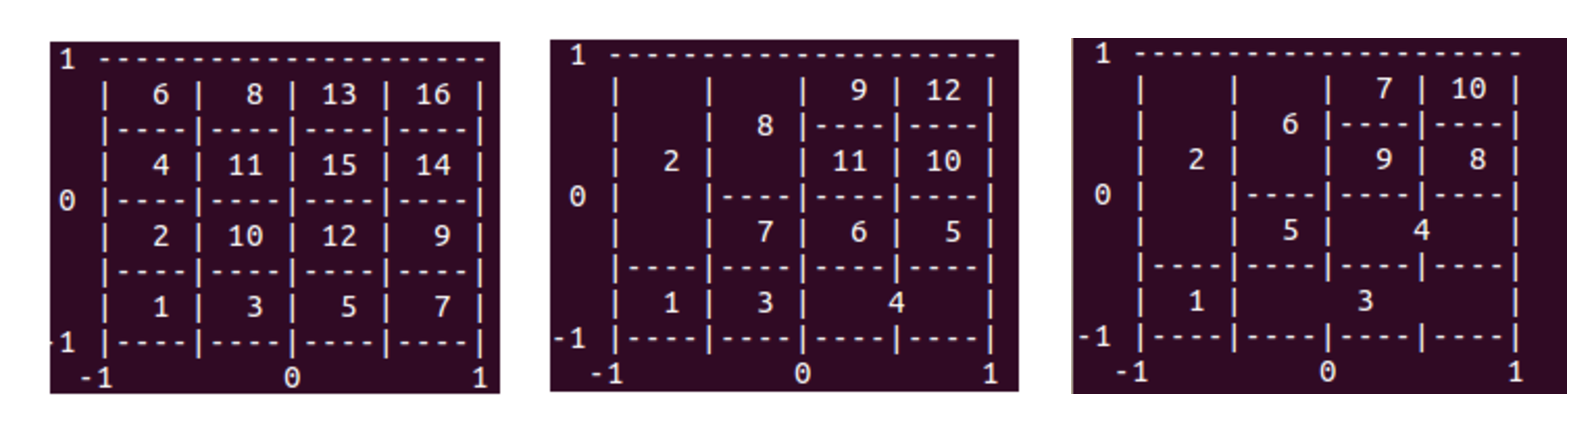
\includegraphics[width=\textwidth]{bin_scheme.pdf} 
\caption{Binning combination scheme.}
\label{bins}
\end{figure}

\begin{table}[h!]
\centering
\begin{tabular}{llllllll}\hline
Number of bins  & \multicolumn{6}{c}{Bin borders}  & Expected limit \\%\hline 
                &$x_1$&$x_2$&$x_3$&$y_1$&$y_2$&$y_3$&\\\hline           
16 (default)    &-0.5 & 0.0 & 0.5 &-0.5 & 0.0 & 0.5 & $<2.91$\\
16              &-0.5 & 0.3 & 0.7 &-0.5 & 0.3 & 0.7 & $<2.83$\\
10              &-0.5 & 0.0 & 0.5 &-0.5 & 0.0 & 0.5 & $<2.93$\\
10              &-0.5 & 0.0 & 0.7 &-0.5 & 0.0 & 0.7 & $<2.86$\\
10              &-0.5 & 0.0 & 0.7 &-0.5 & 0.0 & 0.5 & $<2.84$\\
10              &-0.5 & 0.0 & 0.5 &-0.5 & 0.0 & 0.7 & $<2.87$\\
\textbf{10}     &\textbf{-0.5} &\textbf{0.4} &\textbf{0.7} &\textbf{-0.5} &\textbf{0.4} &\textbf{0.7} &$\mathbf{<2.81}$\\\hline
\end{tabular}
\caption[Limit variation as a function of bin size, $3l$ channel.]{Limit variation as a function of bin size. The final bin borders used in the $3l$ channel are indicated in bold.}
\label{bin_limits}
\end{table}

Combining the optimization of binning and using the tighter pre-selection cuts, the expected limit in the $3l$ channel alone reaches \textbf{r<2.59}.

A similar binning optimization was made for $2lss$ channel, including other binning combinations. First, the $3l$ channel binning was used to estimate the expected limit, then, bin borders were varied to obtain the best possible expected limit. The bin borders and the resulting signal strength limits for the same-sign dimuon channel are shown in Table~\ref{bin_limits_2lss}.

\begin{table}[h!]
\centering
\begin{tabular}{llllllll}\hline
Number of bins  & \multicolumn{6}{c}{Bin borders}  & Expected limit \\
                &$x_1$&$x_2$&$x_3$&$y_1$&$y_2$&$y_3$&\\\hline
16              &-0.5 & 0.4 & 0.7 &-0.5 & 0.4 & 0.7 & $<1.72$\\
12              &-0.5 & 0.4 & 0.7 &-0.5 & 0.4 & 0.7 & $<1.72$\\
12              &-0.3 & 0.4 & 0.7 &-0.5 & 0.4 & 0.7 & $<1.71$\\
12              &-0.3 & 0.3 & 0.7 &-0.5 & 0.4 & 0.7 & $<1.71$\\
12              &-0.3 & 0.3 & 0.7 &-0.4 & 0.4 & 0.7 & $<1.70$\\
12              &-0.3 & 0.3 & 0.7 &-0.3 & 0.4 & 0.7 & $<1.70$\\
12              &-0.3 & 0.3 & 0.7 &-0.3 & 0.2 & 0.7 & $<1.68$\\
12              &-0.3 & 0.3 & 0.7 &-0.3 & 0.1 & 0.7 & $<1.70$\\
12              &-0.3 & 0.3 & 0.7 &-0.3 & 0.2 & 0.6 & $<1.70$\\
10              &-0.5 & 0.4 & 0.7 &-0.5 & 0.4 & 0.7 & $<1.75$\\
\textbf{10}     &\textbf{-0.3} &\textbf{ 0.3} &\textbf{ 0.7} &\textbf{-0.3} &\textbf{ 0.2} &\textbf{ 0.6} &$\mathbf{<1.69}$\\\hline
\end{tabular}
\caption[Limit variation as a function of bin size, $2lss$ channel.]{Limit variation as a function of bin size in the same-sign dimuon channel. (In bold: the final bin borders used in the $2lss$ channel.)}
\label{bin_limits_2lss}
\end{table}

The expected limit was found to be \textbf{r<1.69} for optimized bin borders in 10 bins and optimized pre-selection cuts.

\section{Other binning strategies}
Two additional strategies of clustering regions in the 2D plane of $BDTG_{tt}$ vs $BDTG_{ttV}$ into bins were attempted, following studies done and documented in great detail in Reference~\cite{CMS_AN_2017-029}. A brief description is provided in the following.

\textbf{Clustering by S/B ratio}\\
In this method, the 2D plane is clustered into a given number of bins corresponding to regions where S/B is within a certain range. The bin borders are determined such that the number of background events in each bin is approximately equal. The resulting regions for $2lss$ and $3l$  events are shown in Figure ~\ref{fig:sbbinning}, while the expected distribution of signal and dominant backgrounds are shown in Figure~\ref{fig:sbfinalbins}.

\begin{figure} [!h]
  \centering
  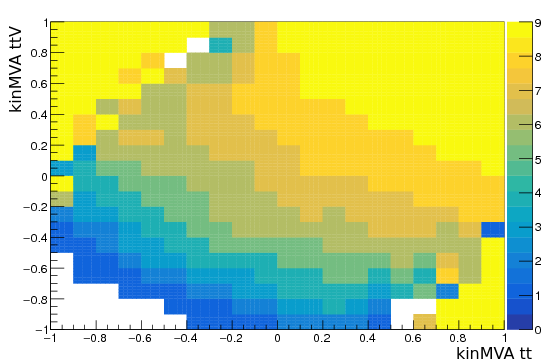
\includegraphics[width=0.45\textwidth]{binning/hTargetBinning_2lss.png}
  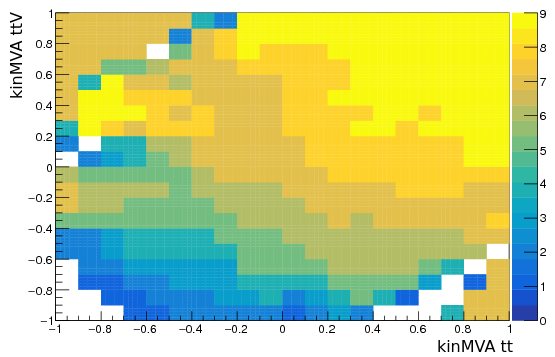
\includegraphics[width=0.45\textwidth]{binning/hTargetBinning_3l.png}
  \caption{Binning by S/B regions for $2lss$ (left) and $3l$ (right).}
  \label{fig:sbbinning}
\end{figure}

\begin{figure} [!h]
  \centering
  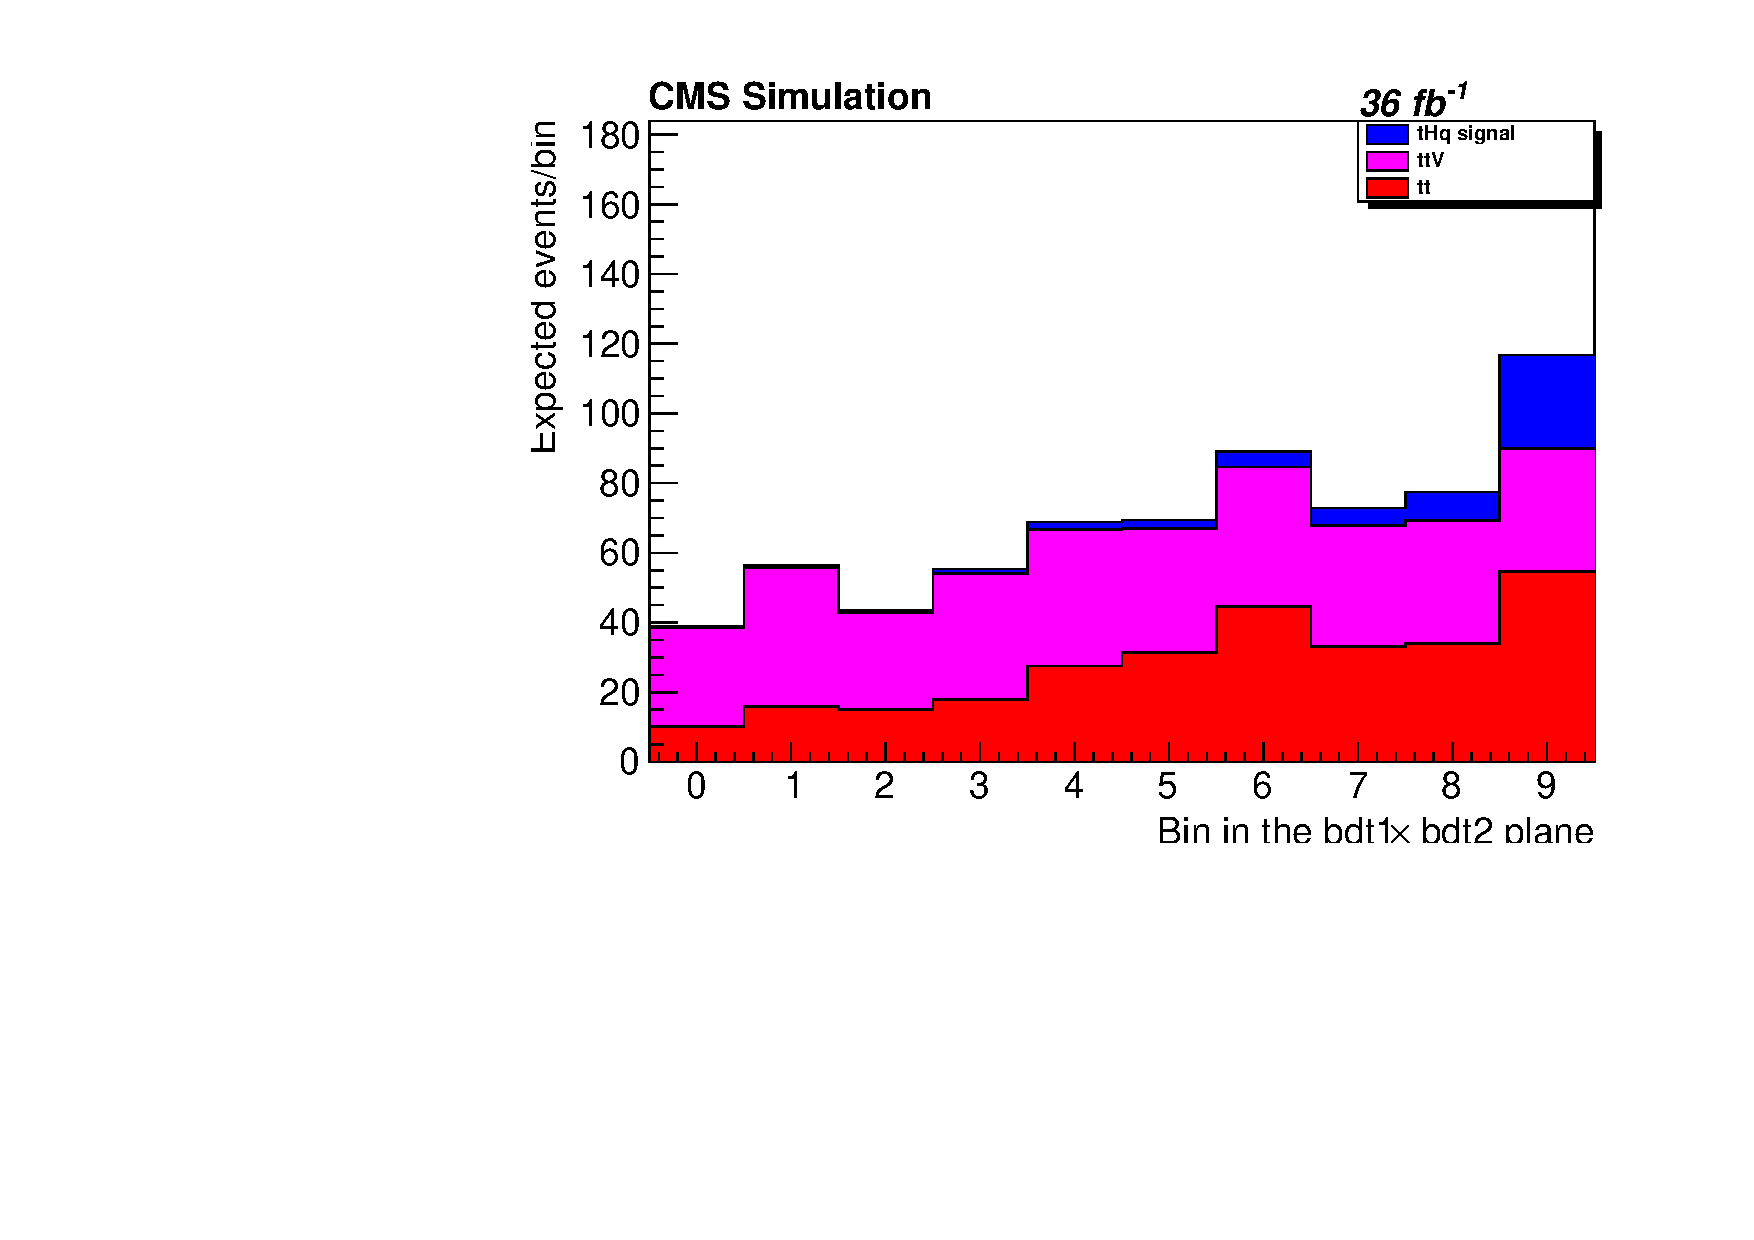
\includegraphics[width=0.45\textwidth]{binning/likelihoodBased_1d_2lss.pdf}
  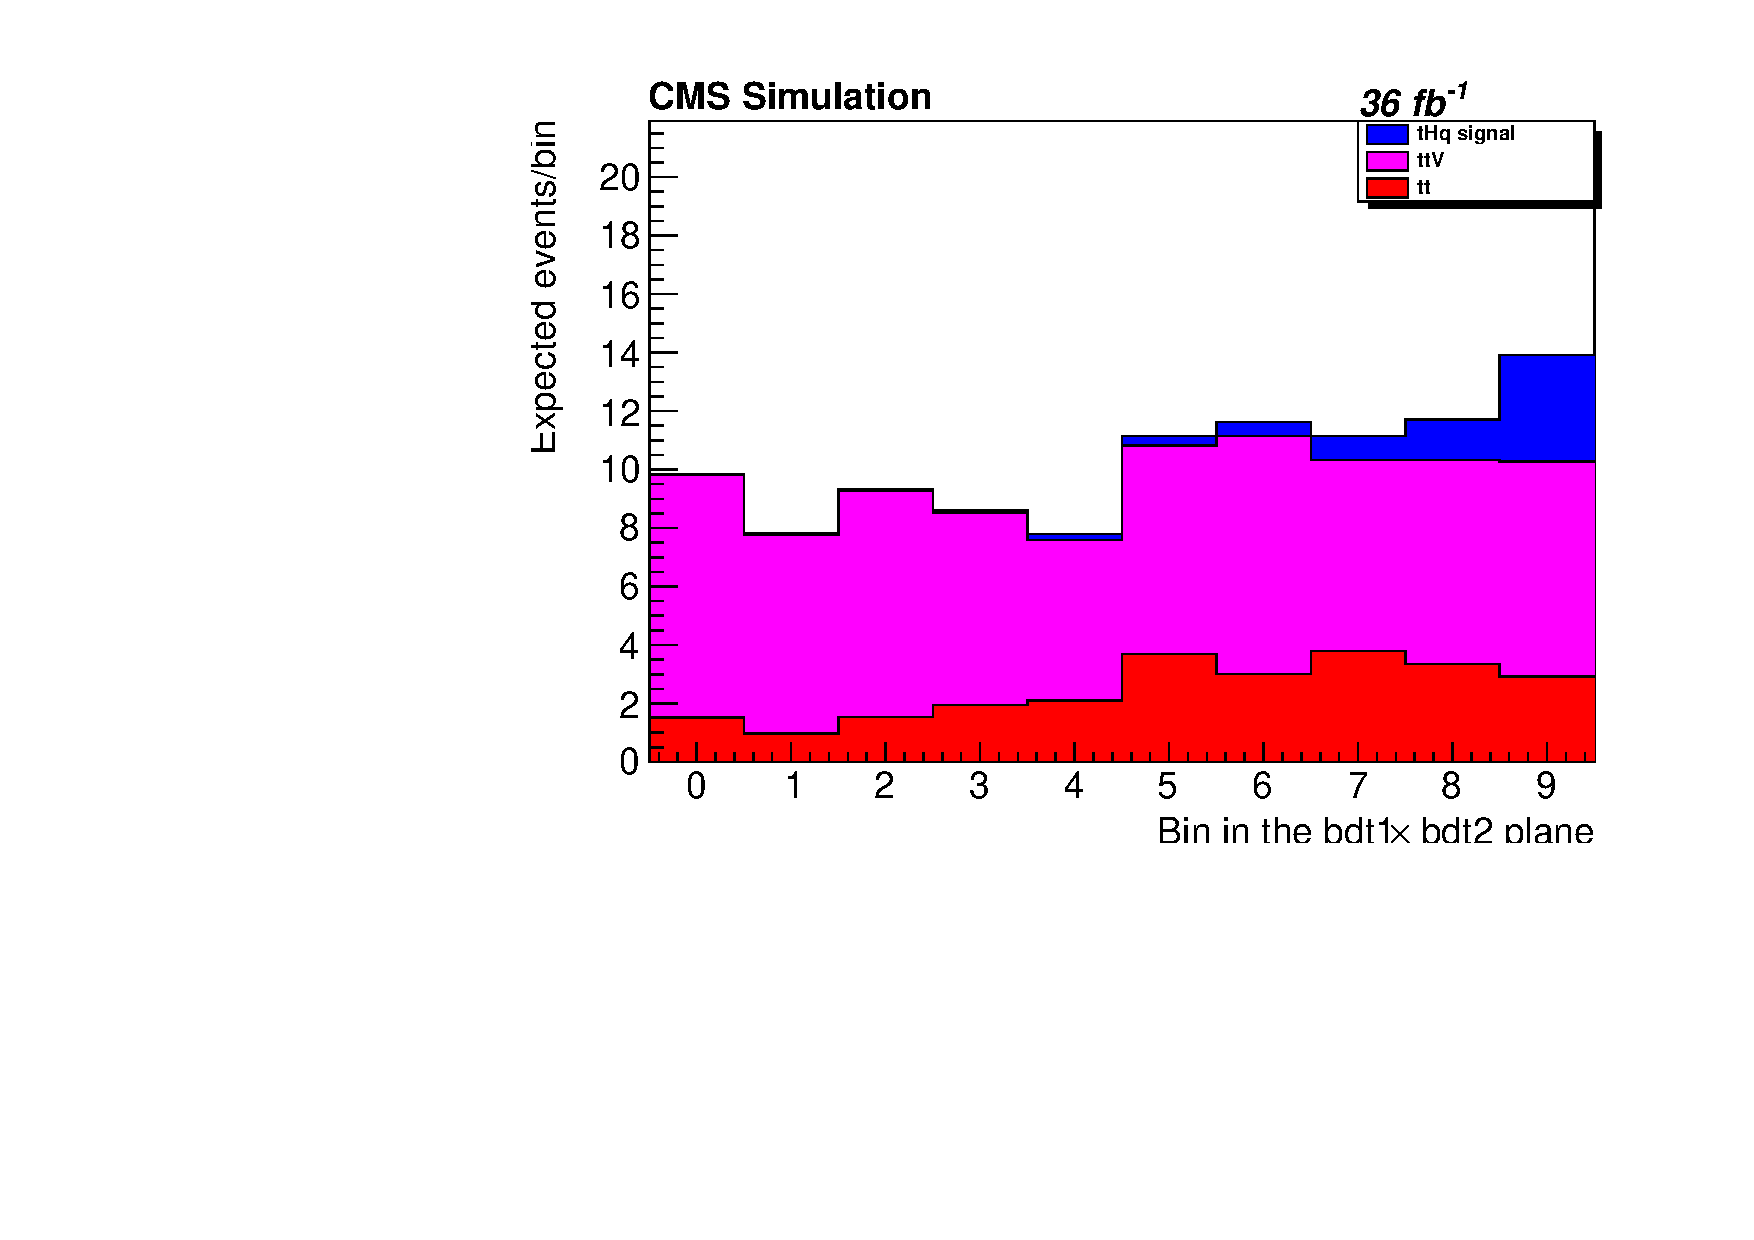
\includegraphics[width=0.45\textwidth]{binning/likelihoodBased_1d_3l.pdf}
  \caption[Final bins (corresponding to S/B regions in the 2D plane)]{Final bins (corresponding to S/B regions in the 2D plane) for $2lss$ and $3l$ (right).}
  \label{fig:sbfinalbins}
\end{figure}

Using this method, the resulting limits (for the $\Ct=-1, \CV=1$ scenario) are about 20\% worse than with the binning in Section \ref{sec:binopt}: \mumu\ changed from 1.82 to 2.15, $3l$ changed from 1.52 to 1.75.

\textbf{$k$-Means geometric clustering}\\
This method employs a recursive application of the $k$-means algorithm (see Appendix D in Reference~\cite{CMS_AN_2017-029}) to separate the 2D plane into geometric regions. The resulting clustering (using the \ttH\ multilepton code on \tHq\ signal and \ttbar\ and \ttV\ background events) is shown in Figure ~\ref{fig:kmeansbinning}. The expected distribution of events for the signal and dominant backgrounds in these bins is shown in Fig.~\ref{fig:kmeansfinalbins}.
\begin{figure} [!h]
  \centering
  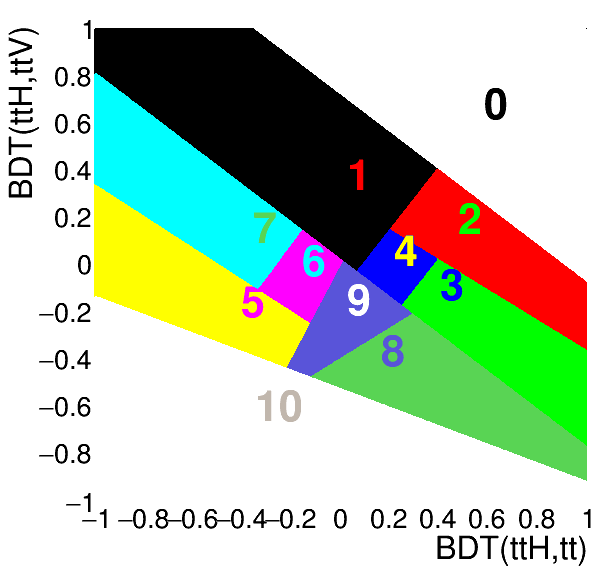
\includegraphics[width=0.45\textwidth]{binning/voronoi_2l_trial0.png}
  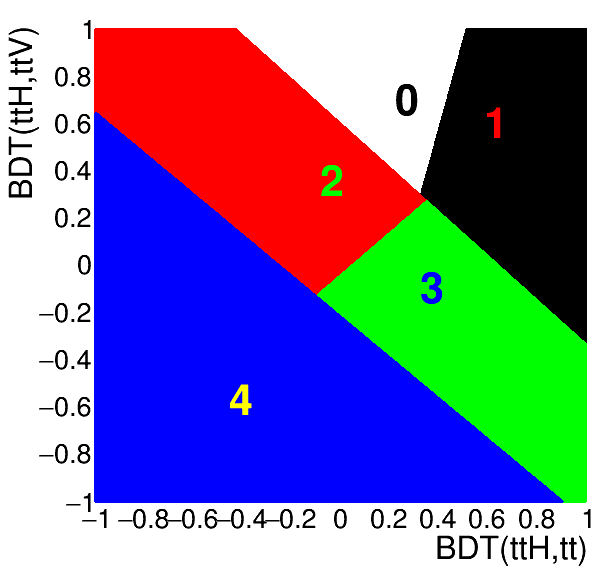
\includegraphics[width=0.45\textwidth]{binning/voronoi_3l_trial0.png}
  \caption[Binning into geometric regions using a $k$-means algorithm.]{Binning into geometric regions using a $k$-means algorithm for $2lss$ (left) and $3l$ (right).}
  \label{fig:kmeansbinning}
\end{figure}

\begin{figure} [!h]
  \centering
  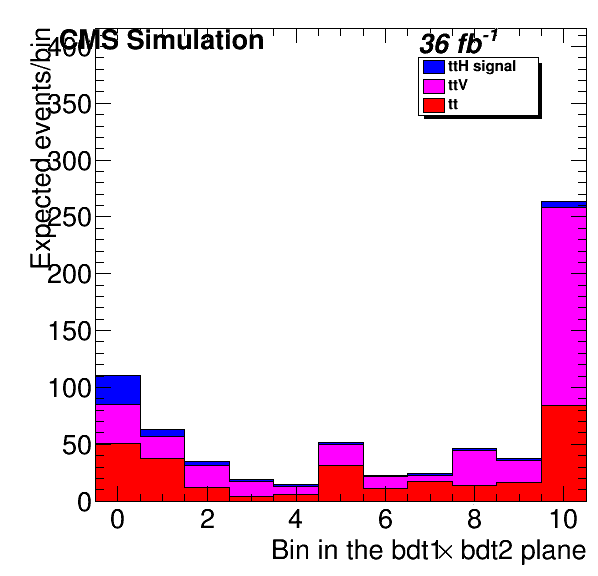
\includegraphics[width=0.45\textwidth]{binning/recursiveNoOrdering_2l_trial0.png}
  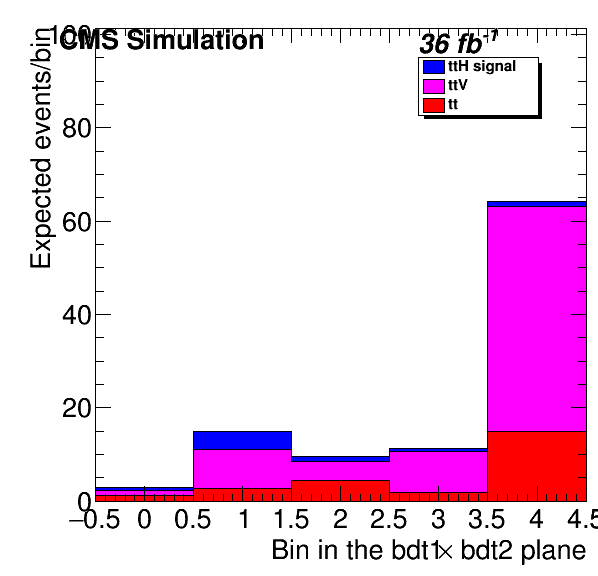
\includegraphics[width=0.45\textwidth]{binning/recursiveNoOrdering_3l_trial0.png}
  \caption[Final bins using a $k$-means algorithm.]{Final bins using a $k$-means algorithm for $2lss$ (left) and $3l$ (right). Note that the bin numbering here is such that signal-like bins are lower.}
  \label{fig:kmeansfinalbins}
\end{figure}

Similarly to the S/B ratio binning, the limits using the $k$-means clustering are significantly worse than those of the bins described before. In the \mumu\ channel, the limit deteriorates from 1.82 to 2.05, whereas in $3l$ it changes from 1.58 to 1.78.
